\documentclass{article}\usepackage[]{graphicx}\usepackage[]{color}
%% maxwidth is the original width if it is less than linewidth
%% otherwise use linewidth (to make sure the graphics do not exceed the margin)
\makeatletter
\def\maxwidth{ %
  \ifdim\Gin@nat@width>\linewidth
    \linewidth
  \else
    \Gin@nat@width
  \fi
}
\makeatother

\definecolor{fgcolor}{rgb}{0.345, 0.345, 0.345}
\newcommand{\hlnum}[1]{\textcolor[rgb]{0.686,0.059,0.569}{#1}}%
\newcommand{\hlstr}[1]{\textcolor[rgb]{0.192,0.494,0.8}{#1}}%
\newcommand{\hlcom}[1]{\textcolor[rgb]{0.678,0.584,0.686}{\textit{#1}}}%
\newcommand{\hlopt}[1]{\textcolor[rgb]{0,0,0}{#1}}%
\newcommand{\hlstd}[1]{\textcolor[rgb]{0.345,0.345,0.345}{#1}}%
\newcommand{\hlkwa}[1]{\textcolor[rgb]{0.161,0.373,0.58}{\textbf{#1}}}%
\newcommand{\hlkwb}[1]{\textcolor[rgb]{0.69,0.353,0.396}{#1}}%
\newcommand{\hlkwc}[1]{\textcolor[rgb]{0.333,0.667,0.333}{#1}}%
\newcommand{\hlkwd}[1]{\textcolor[rgb]{0.737,0.353,0.396}{\textbf{#1}}}%

\usepackage{framed}
\makeatletter
\newenvironment{kframe}{%
 \def\at@end@of@kframe{}%
 \ifinner\ifhmode%
  \def\at@end@of@kframe{\end{minipage}}%
  \begin{minipage}{\columnwidth}%
 \fi\fi%
 \def\FrameCommand##1{\hskip\@totalleftmargin \hskip-\fboxsep
 \colorbox{shadecolor}{##1}\hskip-\fboxsep
     % There is no \\@totalrightmargin, so:
     \hskip-\linewidth \hskip-\@totalleftmargin \hskip\columnwidth}%
 \MakeFramed {\advance\hsize-\width
   \@totalleftmargin\z@ \linewidth\hsize
   \@setminipage}}%
 {\par\unskip\endMakeFramed%
 \at@end@of@kframe}
\makeatother

\definecolor{shadecolor}{rgb}{.97, .97, .97}
\definecolor{messagecolor}{rgb}{0, 0, 0}
\definecolor{warningcolor}{rgb}{1, 0, 1}
\definecolor{errorcolor}{rgb}{1, 0, 0}
\newenvironment{knitrout}{}{} % an empty environment to be redefined in TeX

\usepackage{alltt}
\usepackage[utf8]{inputenc}
\usepackage{amsmath}
\usepackage{graphicx}
%\usepackage{bbold}
\usepackage{tikz}
%\usepackage{silence}
%\WarningFilter{mdframed}{You got a bad break}
\usepackage[colorinlistoftodos]{todonotes}
\usepackage{listings}
\usepackage{color}
\colorlet{exampcol}{blue!10}
\usepackage{multicol}
\usepackage[answerdelayed]{exercise}
\usepackage{booktabs}

\title{BIO311: Population Ecology\\ \textit{Prac 8: Life tables \& Population Matrices}}

\author{Koen van Benthem \& Tina Cornioley\\\\
\tt{koen.vanbenthem@ieu.uzh.ch}\\ \tt{tina.cornioley@ieu.uzh.ch}}

\date{Spring 2014}
\setcounter{tocdepth}{1} % Determines the depth of the table of contents;; 0:chapters, 1: chapters and sections, 2: chapters,sections and subsections

%\renewcommand{\theExercise}{\thechapter.\arabic{Exercise}}%
\IfFileExists{upquote.sty}{\usepackage{upquote}}{}

\begin{document}





\maketitle
\tableofcontents
\vspace{3cm}
\newpage
This is 1 out of 3 methods (so far) for extracting transition rates from the raw data.
\section{Preparing the data}
\begin{knitrout}
\definecolor{shadecolor}{rgb}{0.969, 0.969, 0.969}\color{fgcolor}\begin{kframe}
\begin{alltt}
\hlstd{rot}\hlkwb{<-}\hlkwd{read.csv}\hlstd{(}\hlstr{"rdata.csv"}\hlstd{,}\hlkwc{header}\hlstd{=T,}\hlkwc{sep}\hlstd{=}\hlstr{","}\hlstd{)}
\end{alltt}
\end{kframe}
\end{knitrout}

Since we aim for transitions, rearrange the data, for the transition from timestep 1 to 2:
\begin{knitrout}
\definecolor{shadecolor}{rgb}{0.969, 0.969, 0.969}\color{fgcolor}\begin{kframe}
\begin{alltt}
\hlstd{rot1}\hlkwb{<-}\hlkwd{subset}\hlstd{(rot,Day}\hlopt{==}\hlnum{1}\hlstd{)}
\hlstd{rot2}\hlkwb{<-}\hlkwd{subset}\hlstd{(rot,Day}\hlopt{==}\hlnum{2}\hlstd{)}
\hlstd{rot12}\hlkwb{<-}\hlkwd{merge}\hlstd{(rot1,rot2,}\hlkwc{by}\hlstd{=}\hlkwd{c}\hlstd{(}\hlstr{"Population"}\hlstd{,}\hlstr{"Copper"}\hlstd{,}\hlstr{"Replicate"}\hlstd{))}
\end{alltt}
\end{kframe}
\end{knitrout}

And for the transition from 2 to 3:
\begin{knitrout}
\definecolor{shadecolor}{rgb}{0.969, 0.969, 0.969}\color{fgcolor}\begin{kframe}
\begin{alltt}
\hlstd{rot3}\hlkwb{<-}\hlkwd{subset}\hlstd{(rot,Day}\hlopt{==}\hlnum{3}\hlstd{)}
\hlstd{rot23}\hlkwb{<-}\hlkwd{merge}\hlstd{(rot2,rot3,}\hlkwc{by}\hlstd{=}\hlkwd{c}\hlstd{(}\hlstr{"Population"}\hlstd{,}\hlstr{"Copper"}\hlstd{,}\hlstr{"Replicate"}\hlstd{))}
\end{alltt}
\end{kframe}
\end{knitrout}

And we create one super object that contains all transitions:
\begin{knitrout}
\definecolor{shadecolor}{rgb}{0.969, 0.969, 0.969}\color{fgcolor}\begin{kframe}
\begin{alltt}
\hlstd{rot123}\hlkwb{<-}\hlkwd{rbind}\hlstd{(rot12,rot23)}
\end{alltt}
\end{kframe}
\end{knitrout}

\section{Finding transition rates based on linear fits (\texttt{lm})}
\textit{First we focus only on the transition from timestep 2 to 3}
\begin{kframe}
\begin{alltt}
\hlkwd{library}\hlstd{(}\hlstr{'xtable'}\hlstd{)}
\hlstd{store}\hlkwb{<-}\hlkwd{data.frame}\hlstd{(}\hlkwc{Population}\hlstd{=}\hlkwd{c}\hlstd{(}\hlnum{NA}\hlstd{),}\hlkwc{Copper}\hlstd{=}\hlkwd{c}\hlstd{(}\hlnum{NA}\hlstd{),}\hlkwc{R}\hlstd{=}\hlkwd{c}\hlstd{(}\hlnum{NA}\hlstd{),}\hlkwc{SA}\hlstd{=}\hlkwd{c}\hlstd{(}\hlnum{NA}\hlstd{),}\hlkwc{SJ}\hlstd{=}\hlkwd{c}\hlstd{(}\hlnum{NA}\hlstd{))}
\hlkwa{for}\hlstd{(i} \hlkwa{in} \hlkwd{levels}\hlstd{(rot123}\hlopt{$}\hlstd{Population))\{}
  \hlstd{temp}\hlkwb{<-}\hlkwd{subset}\hlstd{(rot23,Population}\hlopt{==}\hlstd{i)}
  \hlkwa{for}\hlstd{(j} \hlkwa{in} \hlkwd{levels}\hlstd{(rot123}\hlopt{$}\hlstd{Copper))\{}
        \hlcom{# Selecting the correct part of the dataset:}
    \hlstd{temp2}\hlkwb{<-}\hlkwd{subset}\hlstd{(temp,Copper}\hlopt{==}\hlstd{j)}

    \hlkwd{cat}\hlstd{(}\hlstr{"\textbackslash{}\textbackslash{}subsection\{"}\hlstd{,i,j,}\hlstr{"\}\textbackslash{}n"}\hlstd{)}
    \hlkwd{cat}\hlstd{(}\hlstr{"\textbackslash{}\textbackslash{}subsubsection\{Determining reproduction\}\textbackslash{}n\textbackslash{}n"}\hlstd{)}
    \hlkwd{cat}\hlstd{(}\hlstr{"First we fit a value for the reproductive rate using \textbackslash{}\textbackslash{}texttt\{lm\} where we force the line to go through $0$. \textbackslash{}n\textbackslash{}n"}\hlstd{)}

    \hlkwd{par}\hlstd{(}\hlkwc{mar}\hlstd{=}\hlkwd{c}\hlstd{(}\hlnum{6}\hlstd{,}\hlnum{6}\hlstd{,}\hlnum{2}\hlstd{,}\hlnum{2}\hlstd{))}
    \hlkwd{plot}\hlstd{(temp2}\hlopt{$}\hlstd{Alive_Adult.x,temp2}\hlopt{$}\hlstd{Alive_Juv.y,}\hlkwc{xlab}\hlstd{=}\hlstr{"Number of adults at time $t$"}\hlstd{,}\hlkwc{ylab}\hlstd{=}\hlstr{"Number of juveniles at time $t+1$"}\hlstd{,} \hlkwc{main}\hlstd{=}\hlkwd{paste}\hlstd{(}\hlstr{"Reproductive rate"}\hlstd{,i,j),}\hlkwc{xlim}\hlstd{=}\hlkwd{c}\hlstd{(}\hlnum{0}\hlstd{,}\hlkwd{max}\hlstd{(temp2}\hlopt{$}\hlstd{Alive_Adult.x)),}\hlkwc{ylim}\hlstd{=}\hlkwd{c}\hlstd{(}\hlnum{0}\hlstd{,}\hlkwd{max}\hlstd{(temp2}\hlopt{$}\hlstd{Alive_Juv.y)))}
    \hlstd{reg1}\hlkwb{<-}\hlkwd{lm}\hlstd{(temp2}\hlopt{$}\hlstd{Alive_Juv.y}\hlopt{~}\hlstd{temp2}\hlopt{$}\hlstd{Alive_Adult.x}\hlopt{+}\hlnum{0}\hlstd{)}
    \hlkwd{abline}\hlstd{(reg1)}
    \hlkwd{cat}\hlstd{(}\hlstr{"\textbackslash{}n From this regression we found that R="}\hlstd{,reg1}\hlopt{$}\hlstd{coef[[}\hlnum{1}\hlstd{]],}\hlstr{"\textbackslash{}n\textbackslash{}n"}\hlstd{)}

    \hlkwd{cat}\hlstd{(}\hlstr{"\textbackslash{}\textbackslash{}subsubsection\{Determining survival\}\textbackslash{}n\textbackslash{}n"}\hlstd{)}
    \hlkwd{cat}\hlstd{(}\hlstr{"Now we perform a second regression. We fit a plane in which the number of adults next year depends on both the number of juveniles this year and the number of adults this year"}\hlstd{)}
    \hlstd{reg2}\hlkwb{<-}\hlkwd{lm}\hlstd{(temp2}\hlopt{$}\hlstd{Alive_Adult.y}\hlopt{~}\hlstd{temp2}\hlopt{$}\hlstd{Alive_Adult.x}\hlopt{+}\hlstd{temp2}\hlopt{$}\hlstd{Alive_Juv.x}\hlopt{+}\hlnum{0}\hlstd{)}
    \hlkwd{cat}\hlstd{(}\hlstr{"\textbackslash{}\textbackslash{}\textbackslash{}\textbackslash{}From this we find:\textbackslash{}\textbackslash{}\textbackslash{}\textbackslash{} \textbackslash{}n$S_A=$"}\hlstd{,reg2}\hlopt{$}\hlstd{coef[[}\hlnum{1}\hlstd{]],}\hlstr{"\textbackslash{}n$S_J=$"}\hlstd{,reg2}\hlopt{$}\hlstd{coef[[}\hlnum{2}\hlstd{]],}\hlstr{"\textbackslash{}n"}\hlstd{)}

    \hlstd{storet}\hlkwb{<-}\hlkwd{data.frame}\hlstd{(}\hlkwc{Population}\hlstd{=}\hlkwd{c}\hlstd{(i),}\hlkwc{Copper}\hlstd{=}\hlkwd{c}\hlstd{(j),}\hlkwc{R}\hlstd{=}\hlkwd{c}\hlstd{(reg1}\hlopt{$}\hlstd{coef[[}\hlnum{1}\hlstd{]]),}\hlkwc{SA}\hlstd{=}\hlkwd{c}\hlstd{(reg2}\hlopt{$}\hlstd{coef[[}\hlnum{1}\hlstd{]]),}\hlkwc{SJ}\hlstd{=}\hlkwd{c}\hlstd{(reg2}\hlopt{$}\hlstd{coef[[}\hlnum{2}\hlstd{]]))}
    \hlstd{store}\hlkwb{<-}\hlkwd{rbind}\hlstd{(store,storet)}
  \hlstd{\}}

\hlstd{\}}
\end{alltt}
\end{kframe}\subsection{ Commercial high }
\subsubsection{Determining reproduction}

First we fit a value for the reproductive rate using \texttt{lm} where we force the line to go through $0$. 



{\centering 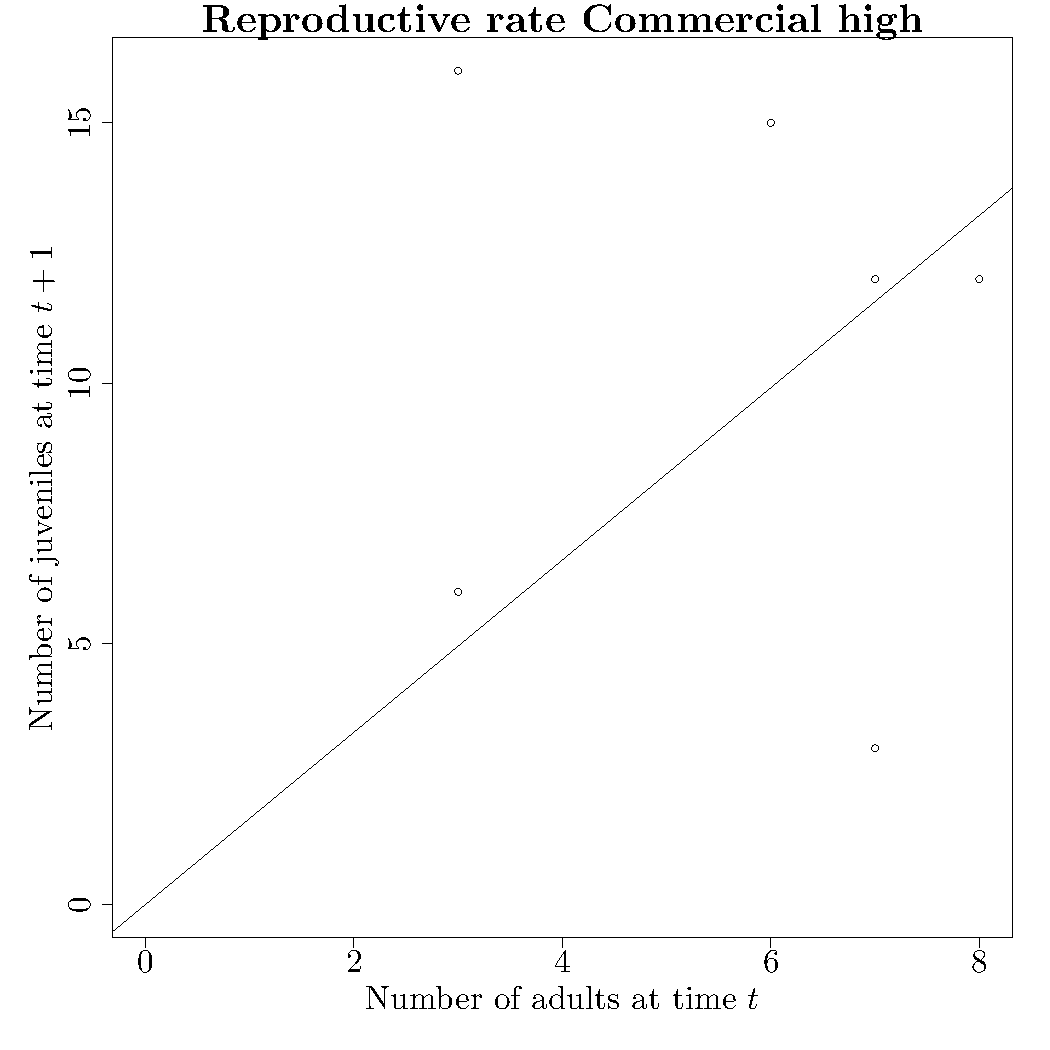
\includegraphics[width=0.65\textwidth]{figure/k51} 

}



 From this regression we found that R= 1.653 

\subsubsection{Determining survival}

Now we perform a second regression. We fit a plane in which the number of adults next year depends on both the number of juveniles this year and the number of adults this year\\From this we find:\\ 
$S_A=$ 1.698 
$S_J=$ 0.5537 
\subsection{ Commercial low }
\subsubsection{Determining reproduction}

First we fit a value for the reproductive rate using \texttt{lm} where we force the line to go through $0$. 



{\centering 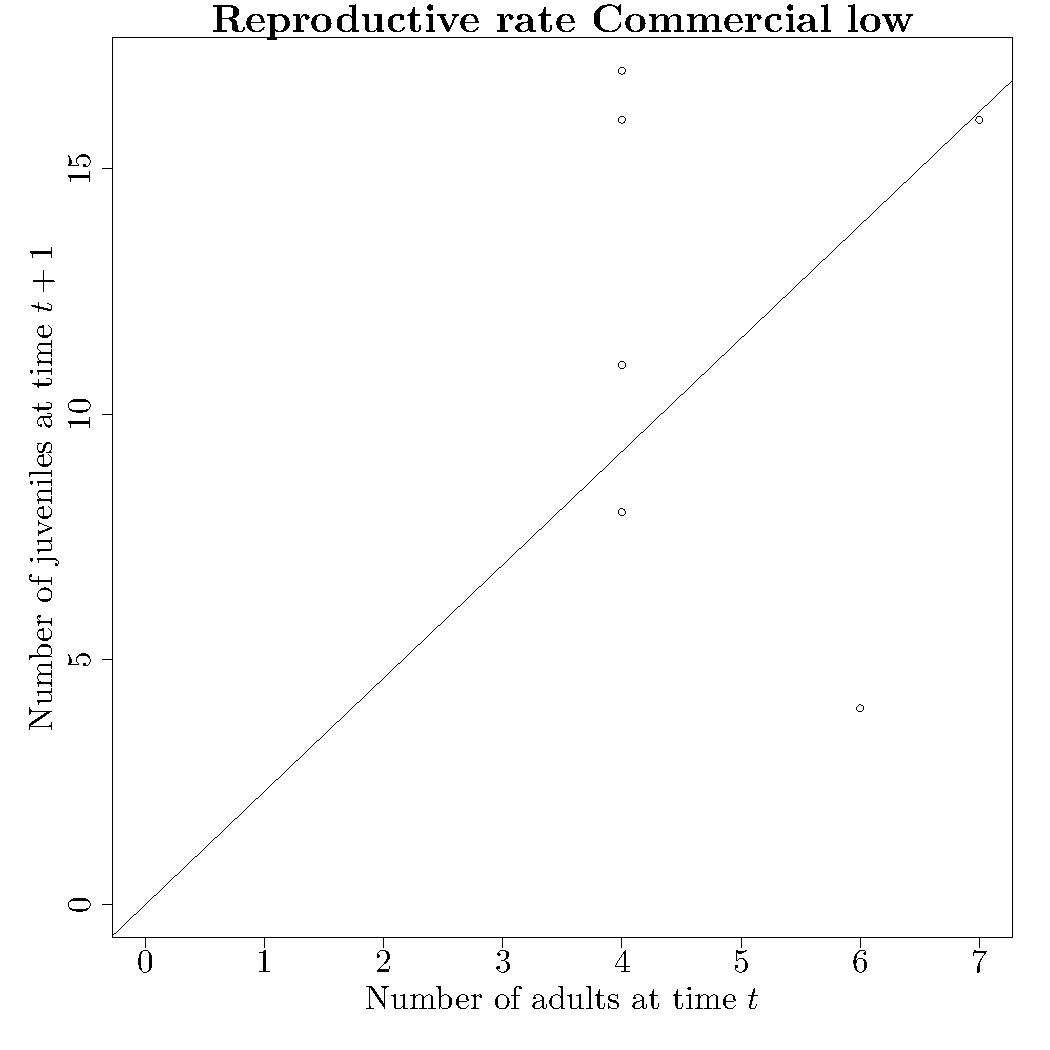
\includegraphics[width=0.65\textwidth]{figure/k52} 

}



 From this regression we found that R= 2.309 

\subsubsection{Determining survival}

Now we perform a second regression. We fit a plane in which the number of adults next year depends on both the number of juveniles this year and the number of adults this year\\From this we find:\\ 
$S_A=$ 0.893 
$S_J=$ 1.039 
\subsection{ Commercial medium }
\subsubsection{Determining reproduction}

First we fit a value for the reproductive rate using \texttt{lm} where we force the line to go through $0$. 



{\centering 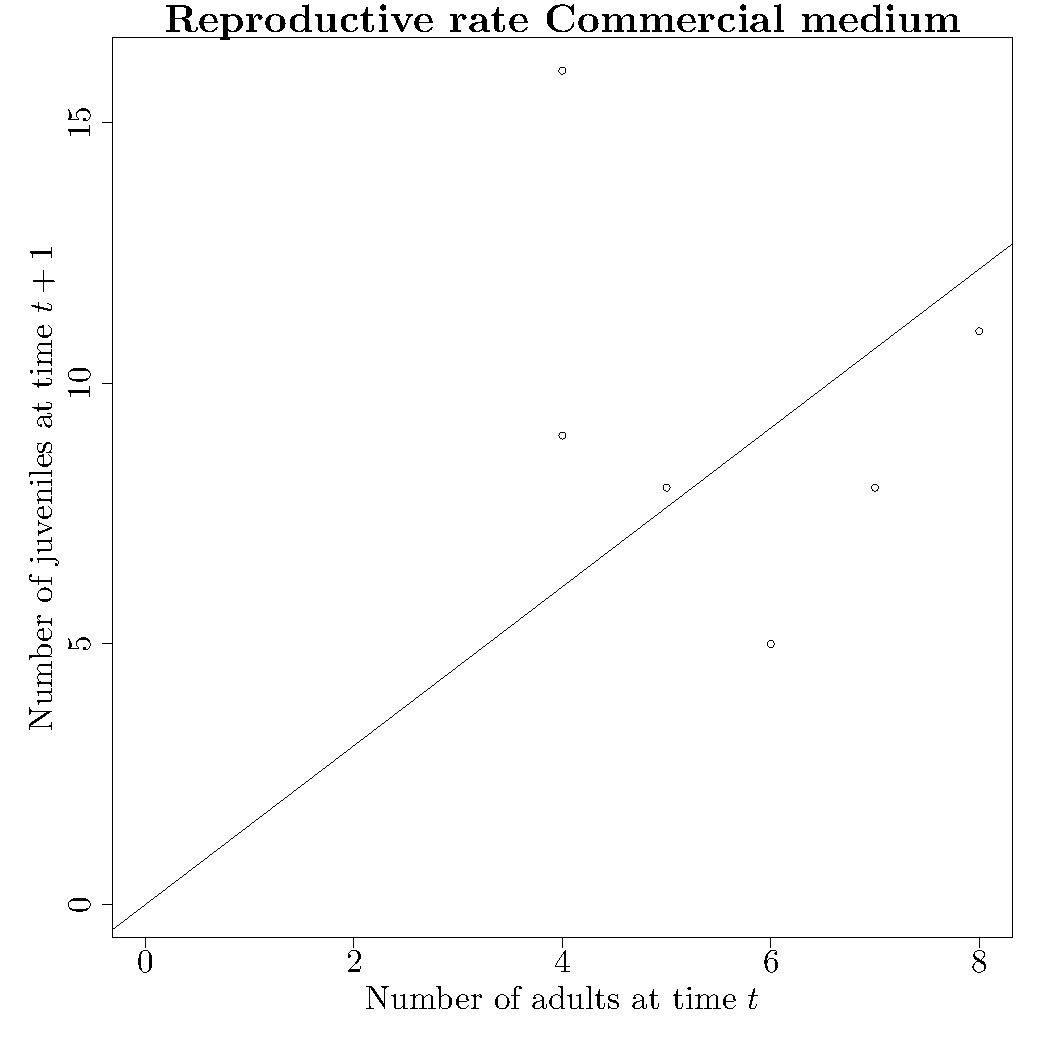
\includegraphics[width=0.65\textwidth]{figure/k53} 

}



 From this regression we found that R= 1.524 

\subsubsection{Determining survival}

Now we perform a second regression. We fit a plane in which the number of adults next year depends on both the number of juveniles this year and the number of adults this year\\From this we find:\\ 
$S_A=$ 1.669 
$S_J=$ 0.3427 
\subsection{ Pollution high }
\subsubsection{Determining reproduction}

First we fit a value for the reproductive rate using \texttt{lm} where we force the line to go through $0$. 



{\centering 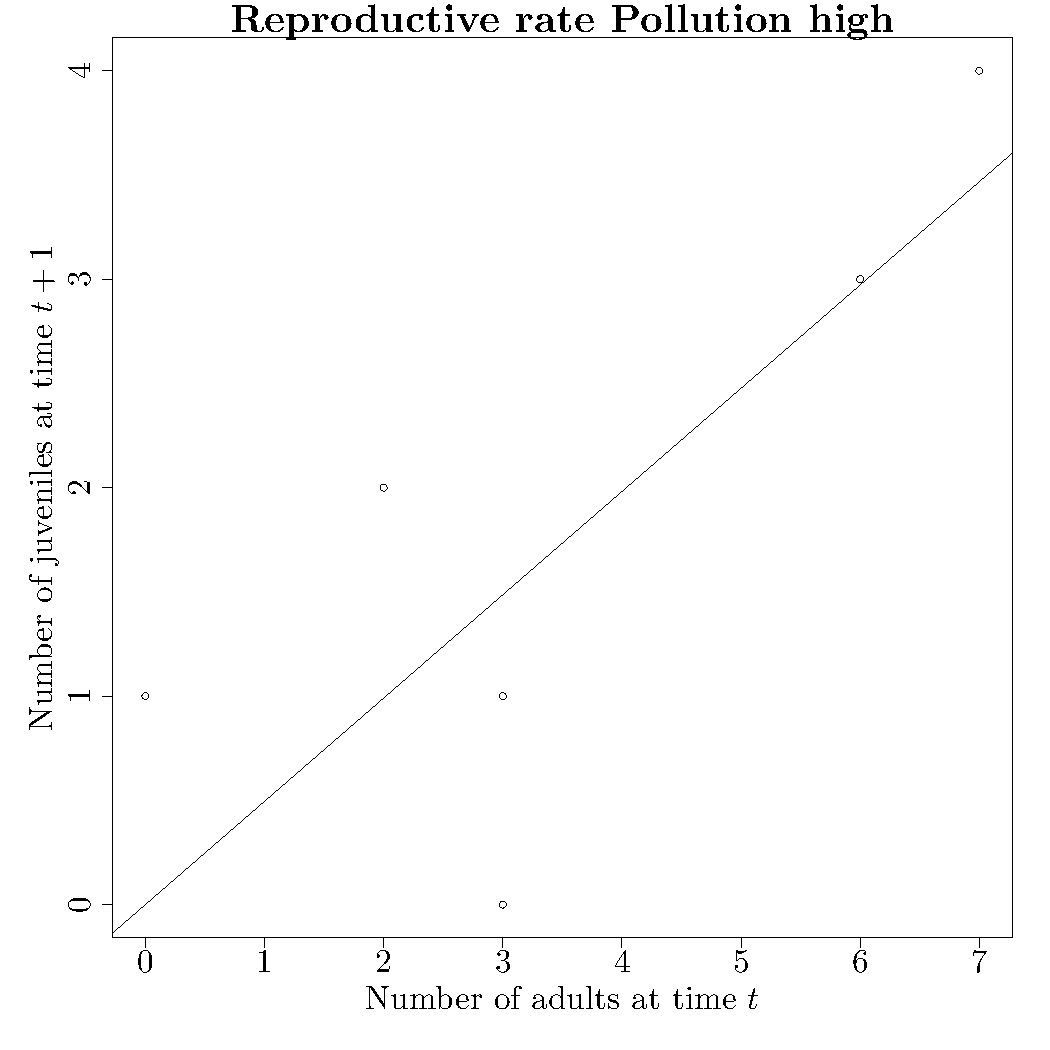
\includegraphics[width=0.65\textwidth]{figure/k54} 

}



 From this regression we found that R= 0.4953 

\subsubsection{Determining survival}

Now we perform a second regression. We fit a plane in which the number of adults next year depends on both the number of juveniles this year and the number of adults this year\\From this we find:\\ 
$S_A=$ 1.295 
$S_J=$ -0.07418 
\subsection{ Pollution low }
\subsubsection{Determining reproduction}

First we fit a value for the reproductive rate using \texttt{lm} where we force the line to go through $0$. 



{\centering 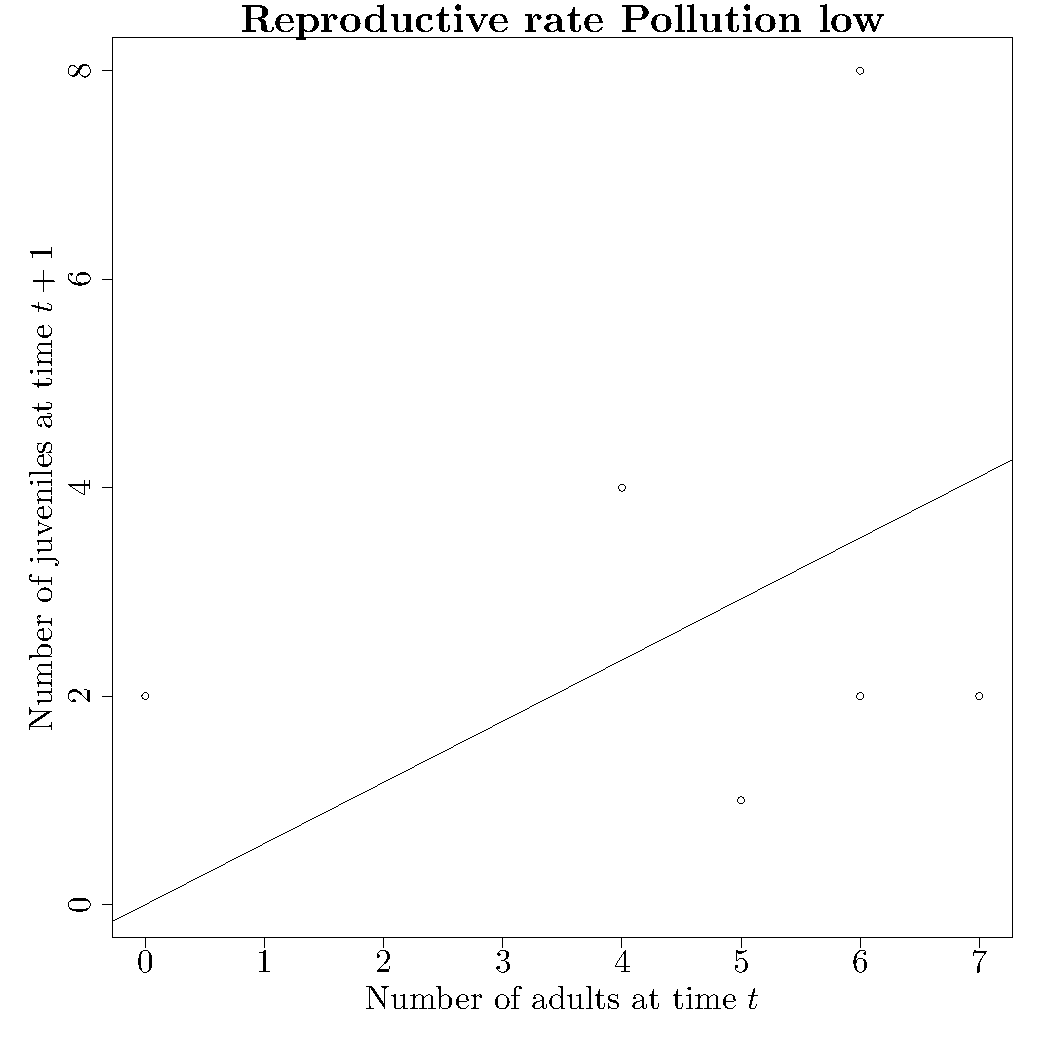
\includegraphics[width=0.65\textwidth]{figure/k55} 

}



 From this regression we found that R= 0.5864 

\subsubsection{Determining survival}

Now we perform a second regression. We fit a plane in which the number of adults next year depends on both the number of juveniles this year and the number of adults this year\\From this we find:\\ 
$S_A=$ 1.373 
$S_J=$ 0.424 
\subsection{ Pollution medium }
\subsubsection{Determining reproduction}

First we fit a value for the reproductive rate using \texttt{lm} where we force the line to go through $0$. 



{\centering 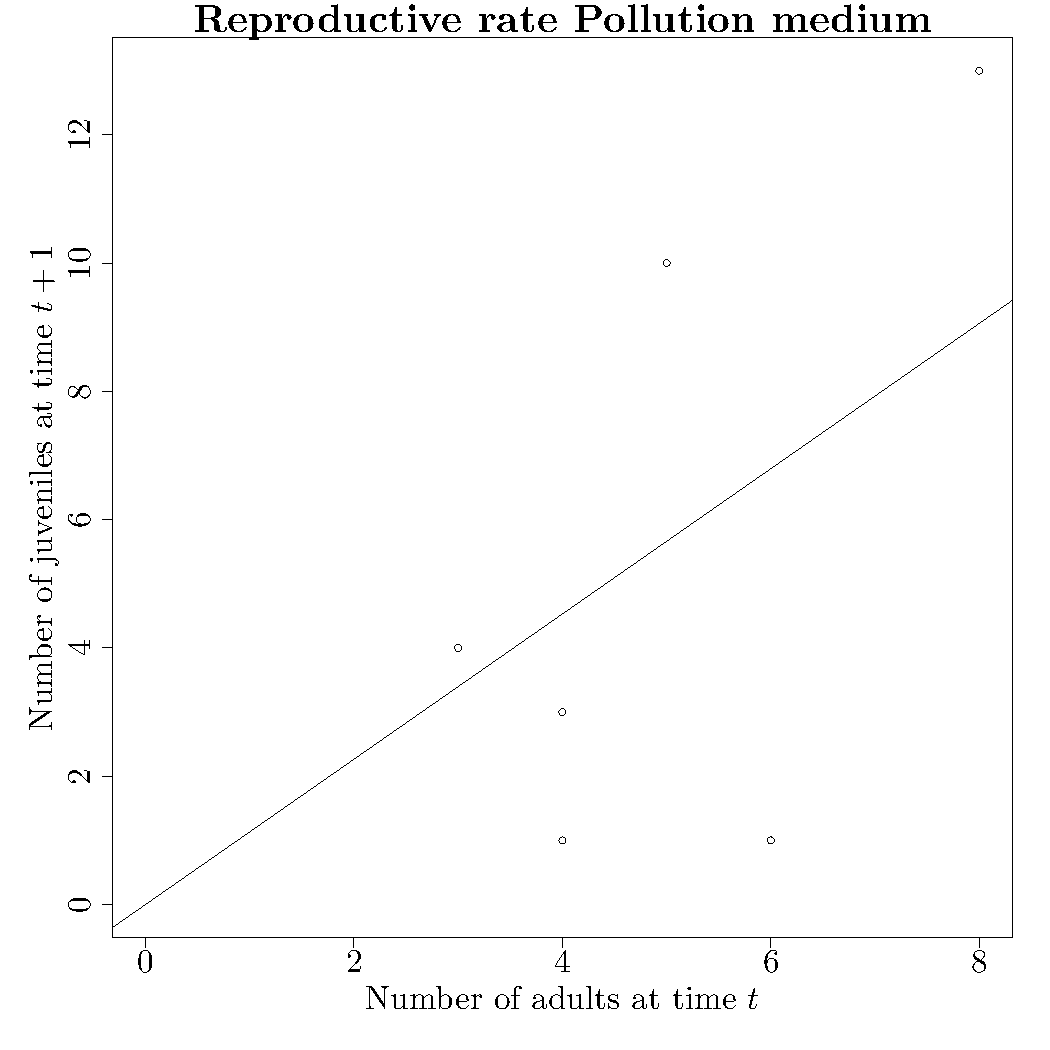
\includegraphics[width=0.65\textwidth]{figure/k56} 

}



 From this regression we found that R= 1.133 

\subsubsection{Determining survival}

Now we perform a second regression. We fit a plane in which the number of adults next year depends on both the number of juveniles this year and the number of adults this year\\From this we find:\\ 
$S_A=$ 1.086 
$S_J=$ -0.08364 
\subsection{ Postpollution high }
\subsubsection{Determining reproduction}

First we fit a value for the reproductive rate using \texttt{lm} where we force the line to go through $0$. 



{\centering 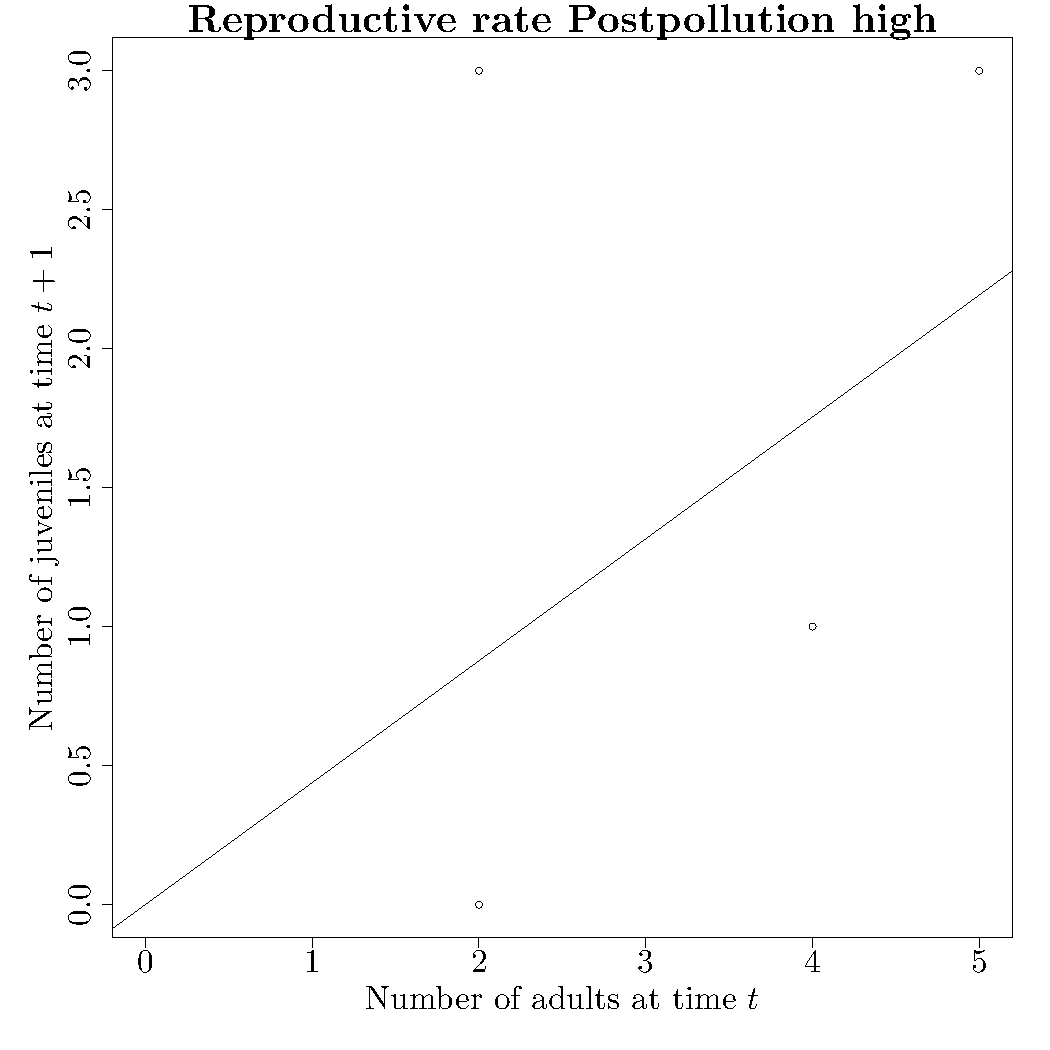
\includegraphics[width=0.65\textwidth]{figure/k57} 

}



 From this regression we found that R= 0.4386 

\subsubsection{Determining survival}

Now we perform a second regression. We fit a plane in which the number of adults next year depends on both the number of juveniles this year and the number of adults this year\\From this we find:\\ 
$S_A=$ 1.024 
$S_J=$ 0.4491 
\subsection{ Postpollution low }
\subsubsection{Determining reproduction}

First we fit a value for the reproductive rate using \texttt{lm} where we force the line to go through $0$. 



{\centering 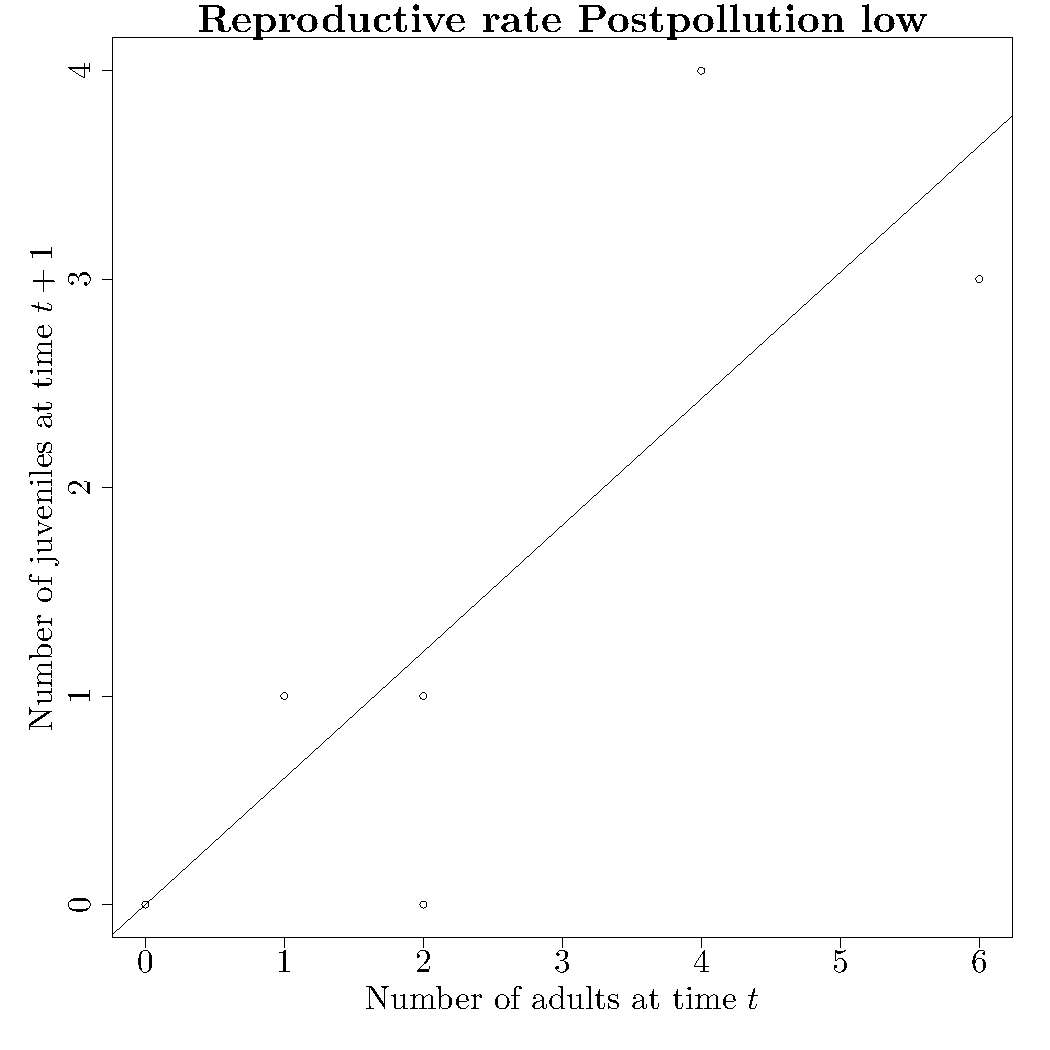
\includegraphics[width=0.65\textwidth]{figure/k58} 

}



 From this regression we found that R= 0.6066 

\subsubsection{Determining survival}

Now we perform a second regression. We fit a plane in which the number of adults next year depends on both the number of juveniles this year and the number of adults this year\\From this we find:\\ 
$S_A=$ 0.07692 
$S_J=$ 4.692 
\subsection{ Postpollution medium }
\subsubsection{Determining reproduction}

First we fit a value for the reproductive rate using \texttt{lm} where we force the line to go through $0$. 



{\centering 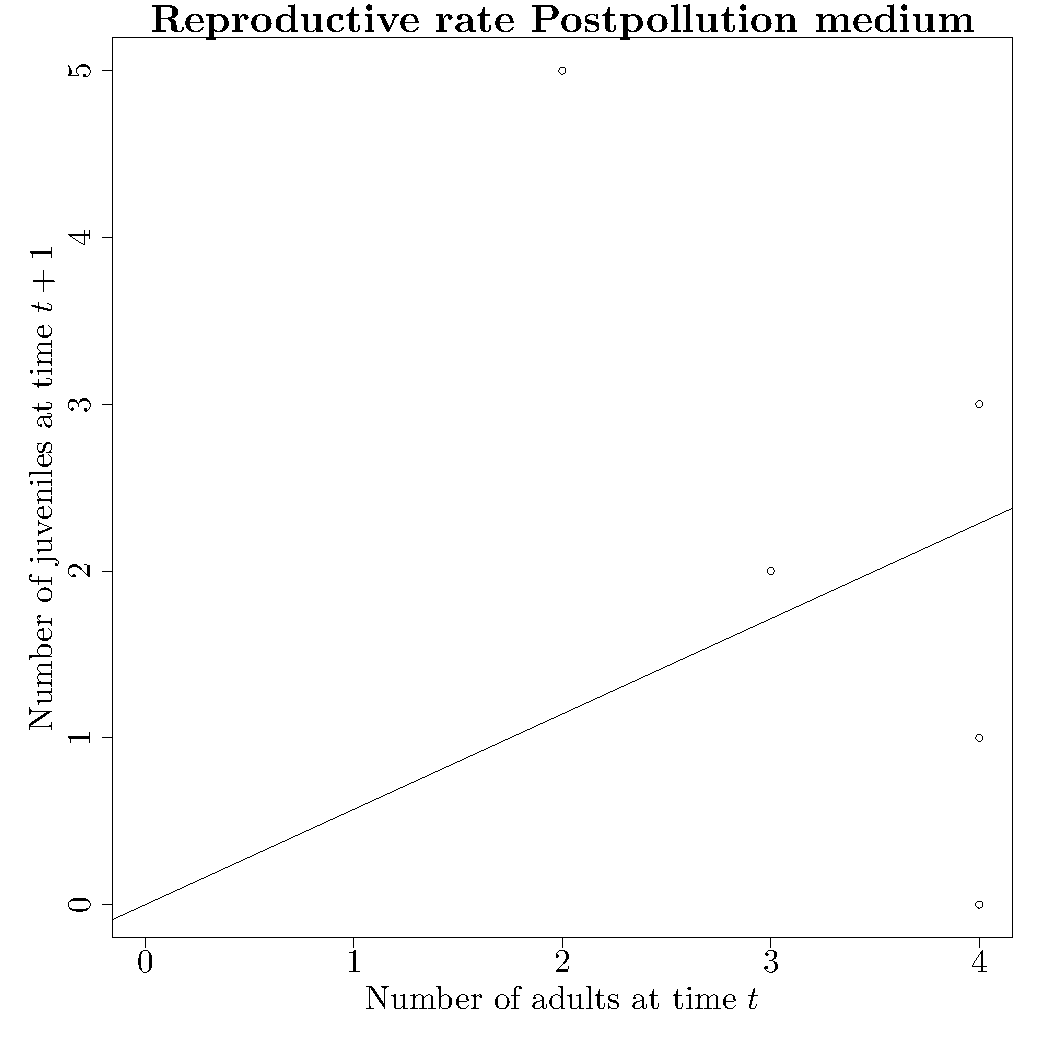
\includegraphics[width=0.65\textwidth]{figure/k59} 

}



 From this regression we found that R= 0.5714 

\subsubsection{Determining survival}

Now we perform a second regression. We fit a plane in which the number of adults next year depends on both the number of juveniles this year and the number of adults this year\\From this we find:\\ 
$S_A=$ 0.8715 
$S_J=$ -0.257 
\subsection{ Recovery high }
\subsubsection{Determining reproduction}

First we fit a value for the reproductive rate using \texttt{lm} where we force the line to go through $0$. 



{\centering 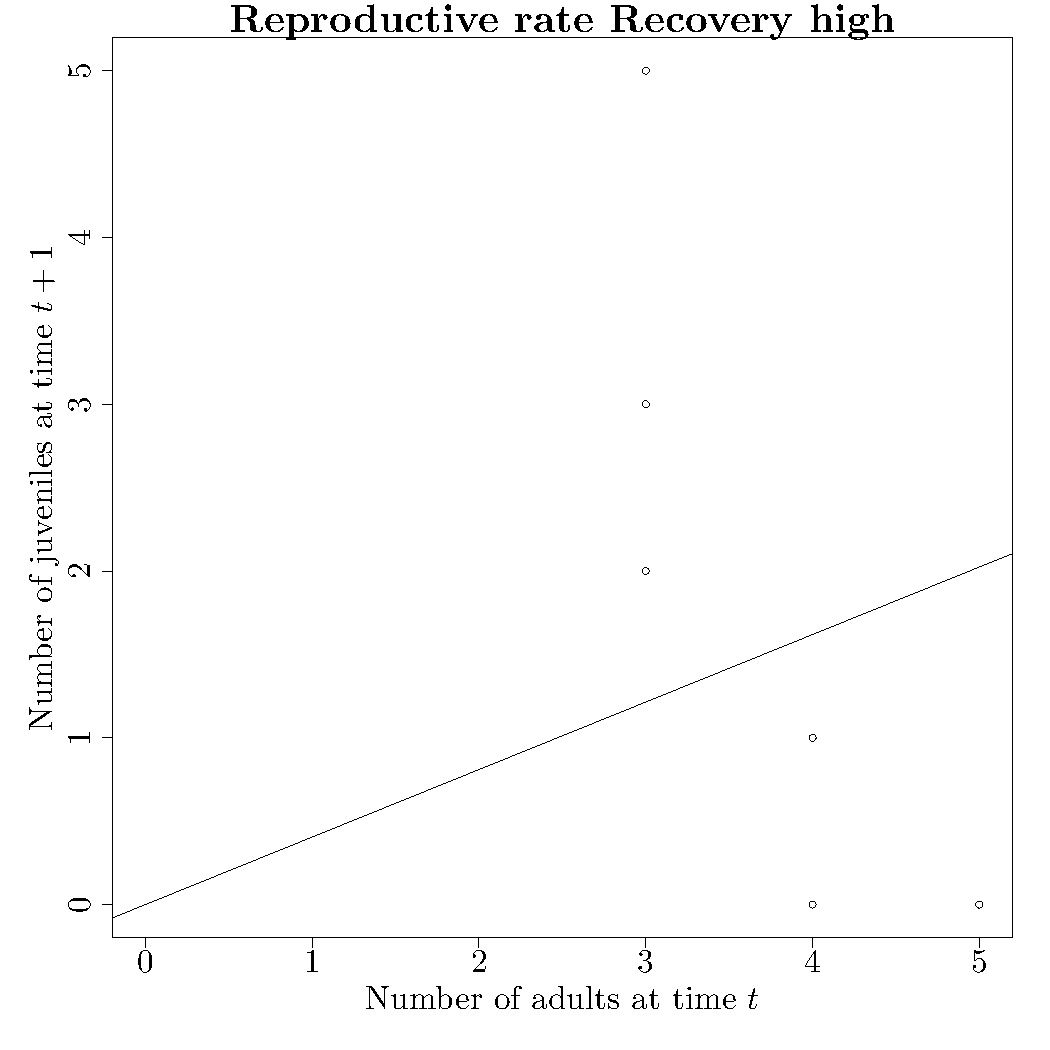
\includegraphics[width=0.65\textwidth]{figure/k510} 

}



 From this regression we found that R= 0.4048 

\subsubsection{Determining survival}

Now we perform a second regression. We fit a plane in which the number of adults next year depends on both the number of juveniles this year and the number of adults this year\\From this we find:\\ 
$S_A=$ 1.097 
$S_J=$ 0.4803 
\subsection{ Recovery low }
\subsubsection{Determining reproduction}

First we fit a value for the reproductive rate using \texttt{lm} where we force the line to go through $0$. 



{\centering 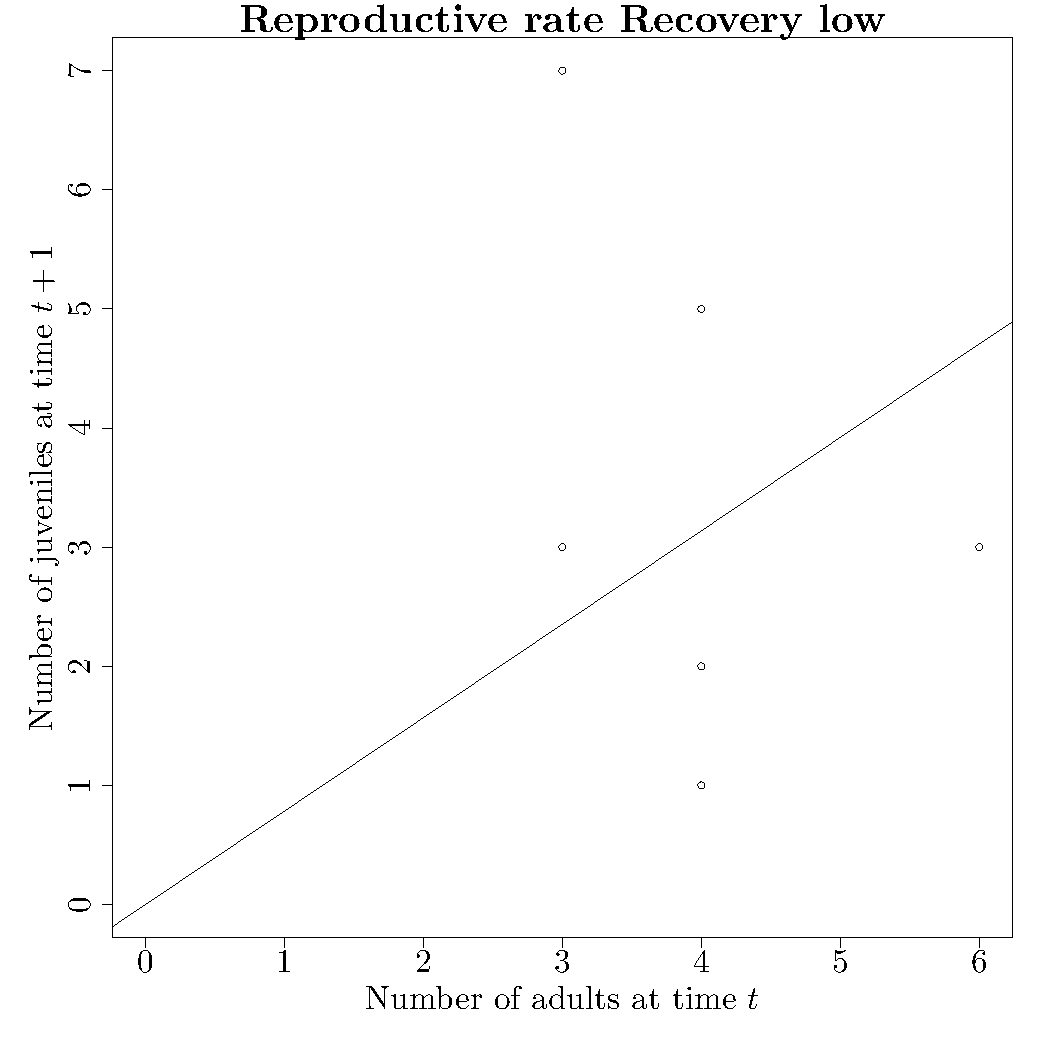
\includegraphics[width=0.65\textwidth]{figure/k511} 

}



 From this regression we found that R= 0.7843 

\subsubsection{Determining survival}

Now we perform a second regression. We fit a plane in which the number of adults next year depends on both the number of juveniles this year and the number of adults this year\\From this we find:\\ 
$S_A=$ 0.8964 
$S_J=$ 0.5193 
\subsection{ Recovery medium }
\subsubsection{Determining reproduction}

First we fit a value for the reproductive rate using \texttt{lm} where we force the line to go through $0$. 



{\centering 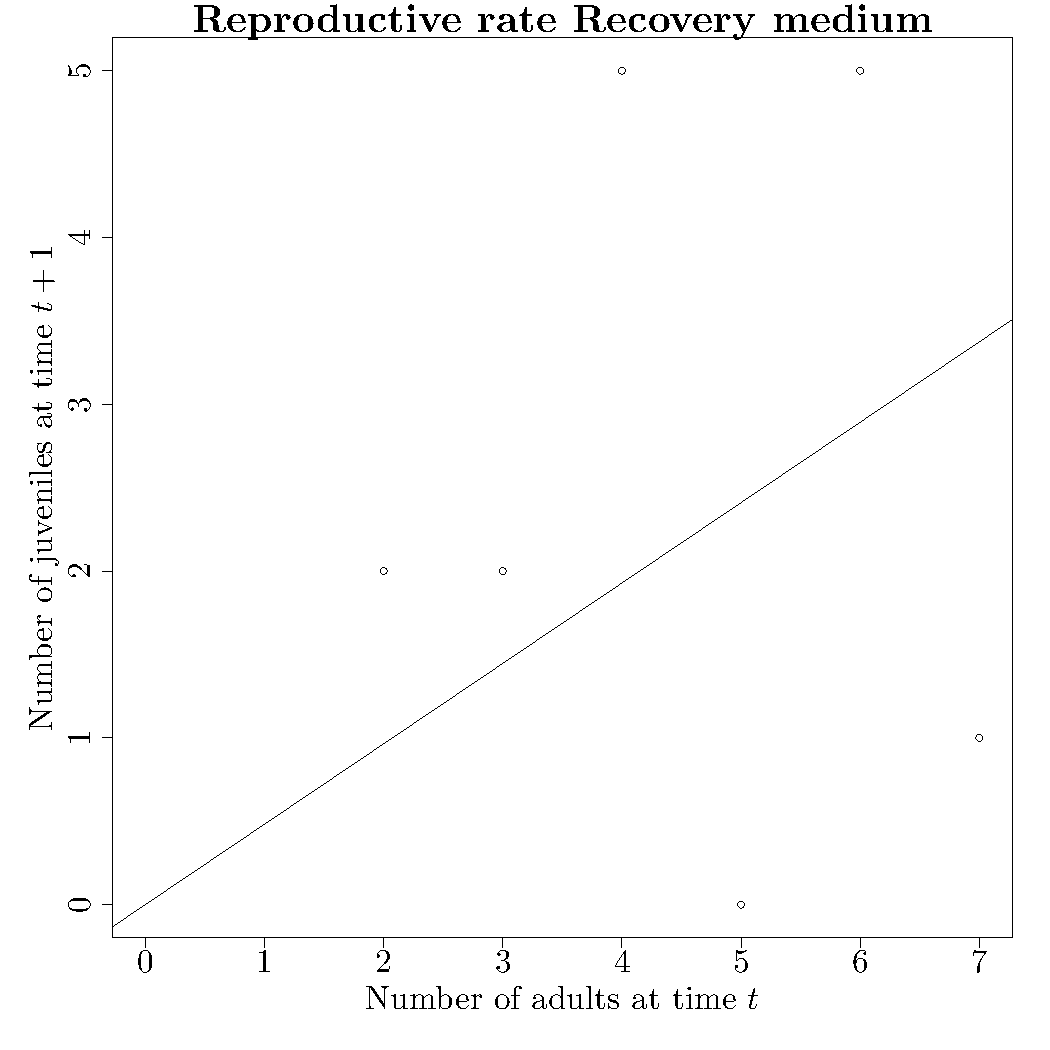
\includegraphics[width=0.65\textwidth]{figure/k512} 

}



 From this regression we found that R= 0.482 

\subsubsection{Determining survival}

Now we perform a second regression. We fit a plane in which the number of adults next year depends on both the number of juveniles this year and the number of adults this year\\From this we find:\\ 
$S_A=$ 1.09 
$S_J=$ -0.1955 
\begin{kframe}\begin{alltt}
\hlkwd{cat}\hlstd{(}\hlstr{"\textbackslash{}\textbackslash{}subsection\{Summary of the data for the 2--3 transition\}"}\hlstd{)}
\end{alltt}
\end{kframe}\subsection{Summary of the data for the 2--3 transition}\begin{kframe}\begin{alltt}
\hlstd{store}\hlkwb{<-}\hlstd{store[}\hlopt{-}\hlnum{1}\hlstd{,]}
\hlkwd{print}\hlstd{(}\hlkwd{xtable}\hlstd{(store,} \hlkwc{digits}\hlstd{=}\hlnum{2}\hlstd{),}
      \hlkwc{size}\hlstd{=}\hlstr{"footnotesize"}\hlstd{,} \hlcom{#Change size; useful for bigger tables}
      \hlkwc{include.rownames}\hlstd{=}\hlnum{FALSE}\hlstd{,} \hlcom{#Don't print rownames}
      \hlkwc{include.colnames}\hlstd{=}\hlnum{FALSE}\hlstd{,} \hlcom{#We create them ourselves}
      \hlkwc{floating}\hlstd{=}\hlnum{FALSE}\hlstd{,}
      \hlkwc{hline.after}\hlstd{=}\hlkwa{NULL}\hlstd{,} \hlcom{#We don't need hline; we use booktabs}
      \hlkwc{add.to.row} \hlstd{=} \hlkwd{list}\hlstd{(}\hlkwc{pos} \hlstd{=} \hlkwd{list}\hlstd{(}\hlopt{-}\hlnum{1}\hlstd{,}
                                   \hlkwd{nrow}\hlstd{(store)),}
                        \hlkwc{command} \hlstd{=} \hlkwd{c}\hlstd{(}\hlkwd{paste}\hlstd{(}\hlstr{"\textbackslash{}\textbackslash{}toprule \textbackslash{}n"}\hlstd{,}
                                          \hlstr{"$Population$ & $Copper$ & $R$ & $S_A$ & $S_J$ \textbackslash{}\textbackslash{}\textbackslash{}\textbackslash{}\textbackslash{}n"}\hlstd{,}
                                          \hlstr{"\textbackslash{}\textbackslash{}midrule \textbackslash{}n"}\hlstd{),}
                                    \hlstr{"\textbackslash{}\textbackslash{}bottomrule \textbackslash{}n"}\hlstd{)}
                        \hlstd{))}
\end{alltt}
\end{kframe}% latex table generated in R 3.0.2 by xtable 1.7-3 package
% Tue Apr 22 13:23:33 2014
{\footnotesize
\begin{tabular}{llrrr}
  \toprule 
 $Population$ & $Copper$ & $R$ & $S_A$ & $S_J$ \\
 \midrule 
 Commercial & high & 1.65 & 1.70 & 0.55 \\ 
  Commercial & low & 2.31 & 0.89 & 1.04 \\ 
  Commercial & medium & 1.52 & 1.67 & 0.34 \\ 
  Pollution & high & 0.50 & 1.30 & -0.07 \\ 
  Pollution & low & 0.59 & 1.37 & 0.42 \\ 
  Pollution & medium & 1.13 & 1.09 & -0.08 \\ 
  Postpollution & high & 0.44 & 1.02 & 0.45 \\ 
  Postpollution & low & 0.61 & 0.08 & 4.69 \\ 
  Postpollution & medium & 0.57 & 0.87 & -0.26 \\ 
  Recovery & high & 0.40 & 1.10 & 0.48 \\ 
  Recovery & low & 0.78 & 0.90 & 0.52 \\ 
  Recovery & medium & 0.48 & 1.09 & -0.20 \\ 
   \bottomrule 
\end{tabular}
}
\begin{kframe}\begin{alltt}
\hlkwd{cat}\hlstd{(}\hlstr{"\textbackslash{}\textbackslash{}subsection\{Summary of the data for both transitions\}"}\hlstd{)}
\end{alltt}
\end{kframe}\subsection{Summary of the data for both transitions}\begin{kframe}\begin{alltt}
\hlstd{store}\hlkwb{<-}\hlkwd{data.frame}\hlstd{(}\hlkwc{Population}\hlstd{=}\hlkwd{c}\hlstd{(}\hlnum{NA}\hlstd{),}\hlkwc{Copper}\hlstd{=}\hlkwd{c}\hlstd{(}\hlnum{NA}\hlstd{),}\hlkwc{R}\hlstd{=}\hlkwd{c}\hlstd{(}\hlnum{NA}\hlstd{),}\hlkwc{SA}\hlstd{=}\hlkwd{c}\hlstd{(}\hlnum{NA}\hlstd{),}\hlkwc{SJ}\hlstd{=}\hlkwd{c}\hlstd{(}\hlnum{NA}\hlstd{))}
\hlkwa{for}\hlstd{(i} \hlkwa{in} \hlkwd{levels}\hlstd{(rot123}\hlopt{$}\hlstd{Population))\{}
  \hlstd{temp}\hlkwb{<-}\hlkwd{subset}\hlstd{(rot123,Population}\hlopt{==}\hlstd{i)}
  \hlkwa{for}\hlstd{(j} \hlkwa{in} \hlkwd{levels}\hlstd{(rot123}\hlopt{$}\hlstd{Copper))\{}
        \hlcom{# Selecting the correct part of the dataset:}
    \hlstd{temp2}\hlkwb{<-}\hlkwd{subset}\hlstd{(temp,Copper}\hlopt{==}\hlstd{j)}
    \hlstd{reg1}\hlkwb{<-}\hlkwd{lm}\hlstd{(temp2}\hlopt{$}\hlstd{Alive_Juv.y}\hlopt{~}\hlstd{temp2}\hlopt{$}\hlstd{Alive_Adult.x}\hlopt{+}\hlnum{0}\hlstd{)}
    \hlstd{reg2}\hlkwb{<-}\hlkwd{lm}\hlstd{(temp2}\hlopt{$}\hlstd{Alive_Adult.y}\hlopt{~}\hlstd{temp2}\hlopt{$}\hlstd{Alive_Adult.x}\hlopt{+}\hlstd{temp2}\hlopt{$}\hlstd{Alive_Juv.x}\hlopt{+}\hlnum{0}\hlstd{)}

    \hlstd{storet}\hlkwb{<-}\hlkwd{data.frame}\hlstd{(}\hlkwc{Population}\hlstd{=}\hlkwd{c}\hlstd{(i),}\hlkwc{Copper}\hlstd{=}\hlkwd{c}\hlstd{(j),}\hlkwc{R}\hlstd{=}\hlkwd{c}\hlstd{(reg1}\hlopt{$}\hlstd{coef[[}\hlnum{1}\hlstd{]]),}\hlkwc{SA}\hlstd{=}\hlkwd{c}\hlstd{(reg2}\hlopt{$}\hlstd{coef[[}\hlnum{1}\hlstd{]]),}\hlkwc{SJ}\hlstd{=}\hlkwd{c}\hlstd{(reg2}\hlopt{$}\hlstd{coef[[}\hlnum{2}\hlstd{]]))}
    \hlstd{store}\hlkwb{<-}\hlkwd{rbind}\hlstd{(store,storet)}
  \hlstd{\}}

\hlstd{\}}
\hlstd{store}\hlkwb{<-}\hlstd{store[}\hlopt{-}\hlnum{1}\hlstd{,]}
\hlkwd{print}\hlstd{(}\hlkwd{xtable}\hlstd{(store,} \hlkwc{digits}\hlstd{=}\hlnum{2}\hlstd{),}
      \hlkwc{size}\hlstd{=}\hlstr{"footnotesize"}\hlstd{,} \hlcom{#Change size; useful for bigger tables}
      \hlkwc{include.rownames}\hlstd{=}\hlnum{FALSE}\hlstd{,} \hlcom{#Don't print rownames}
      \hlkwc{include.colnames}\hlstd{=}\hlnum{FALSE}\hlstd{,} \hlcom{#We create them ourselves}
      \hlkwc{floating}\hlstd{=}\hlnum{FALSE}\hlstd{,}
      \hlkwc{hline.after}\hlstd{=}\hlkwa{NULL}\hlstd{,} \hlcom{#We don't need hline; we use booktabs}
      \hlkwc{add.to.row} \hlstd{=} \hlkwd{list}\hlstd{(}\hlkwc{pos} \hlstd{=} \hlkwd{list}\hlstd{(}\hlopt{-}\hlnum{1}\hlstd{,}
                                   \hlkwd{nrow}\hlstd{(store)),}
                        \hlkwc{command} \hlstd{=} \hlkwd{c}\hlstd{(}\hlkwd{paste}\hlstd{(}\hlstr{"\textbackslash{}\textbackslash{}toprule \textbackslash{}n"}\hlstd{,}
                                          \hlstr{"$Population$ & $Copper$ & $R$ & $S_A$ & $S_J$ \textbackslash{}\textbackslash{}\textbackslash{}\textbackslash{}\textbackslash{}n"}\hlstd{,}
                                          \hlstr{"\textbackslash{}\textbackslash{}midrule \textbackslash{}n"}\hlstd{),}
                                    \hlstr{"\textbackslash{}\textbackslash{}bottomrule \textbackslash{}n"}\hlstd{)}
                        \hlstd{))}
\end{alltt}
\end{kframe}% latex table generated in R 3.0.2 by xtable 1.7-3 package
% Tue Apr 22 13:23:33 2014
{\footnotesize
\begin{tabular}{llrrr}
  \toprule 
 $Population$ & $Copper$ & $R$ & $S_A$ & $S_J$ \\
 \midrule 
 Commercial & high & 1.59 & 1.72 & 0.42 \\ 
  Commercial & low & 2.26 & 0.75 & 1.09 \\ 
  Commercial & medium & 1.55 & 1.66 & 0.32 \\ 
  Pollution & high & 0.48 & 1.31 & -0.13 \\ 
  Pollution & low & 0.59 & 1.40 & 0.24 \\ 
  Pollution & medium & 1.09 & 0.79 & 0.61 \\ 
  Postpollution & high & 0.40 & 1.15 & -0.10 \\ 
  Postpollution & low & 0.40 & 0.95 & -0.04 \\ 
  Postpollution & medium & 0.69 & 0.76 & 0.09 \\ 
  Recovery & high & 0.62 & 1.14 & 0.29 \\ 
  Recovery & low & 0.78 & 0.94 & 0.42 \\ 
  Recovery & medium & 0.36 & 1.05 & 0.30 \\ 
   \bottomrule 
\end{tabular}
}


\section{Taking into account that $0<S_J<1$ and $0<S_A<1$}
We now use \texttt{nls()} to ensure that both $S_J$ and $S_A$ stay between 0 and 1. (not sure if this is the best solution, but at least it is a solution.) 
\begin{kframe}
\begin{alltt}
\hlkwd{library}\hlstd{(}\hlstr{'xtable'}\hlstd{)}
\hlstd{store}\hlkwb{<-}\hlkwd{data.frame}\hlstd{(}\hlkwc{Population}\hlstd{=}\hlkwd{c}\hlstd{(}\hlnum{NA}\hlstd{),}\hlkwc{Copper}\hlstd{=}\hlkwd{c}\hlstd{(}\hlnum{NA}\hlstd{),}\hlkwc{R}\hlstd{=}\hlkwd{c}\hlstd{(}\hlnum{NA}\hlstd{),}\hlkwc{SA}\hlstd{=}\hlkwd{c}\hlstd{(}\hlnum{NA}\hlstd{),}\hlkwc{SJ}\hlstd{=}\hlkwd{c}\hlstd{(}\hlnum{NA}\hlstd{))}
\hlkwa{for}\hlstd{(i} \hlkwa{in} \hlkwd{levels}\hlstd{(rot123}\hlopt{$}\hlstd{Population))\{}
  \hlstd{temp}\hlkwb{<-}\hlkwd{subset}\hlstd{(rot123,Population}\hlopt{==}\hlstd{i)}
  \hlkwa{for}\hlstd{(j} \hlkwa{in} \hlkwd{levels}\hlstd{(rot123}\hlopt{$}\hlstd{Copper))\{}
        \hlcom{# Selecting the correct part of the dataset:}
    \hlstd{temp2}\hlkwb{<-}\hlkwd{subset}\hlstd{(temp,Copper}\hlopt{==}\hlstd{j)}
    \hlstd{reg1}\hlkwb{<-}\hlkwd{lm}\hlstd{(temp2}\hlopt{$}\hlstd{Alive_Juv.y}\hlopt{~}\hlstd{temp2}\hlopt{$}\hlstd{Alive_Adult.x}\hlopt{+}\hlnum{0}\hlstd{)}
    \hlstd{y}\hlkwb{<-}\hlstd{temp2}\hlopt{$}\hlstd{Alive_Adult.y}
    \hlstd{x1}\hlkwb{<-}\hlstd{temp2}\hlopt{$}\hlstd{Alive_Adult.x}
    \hlstd{x2}\hlkwb{<-}\hlstd{temp2}\hlopt{$}\hlstd{Alive_Juv.x}
    \hlstd{nlsfit}\hlkwb{<-}\hlkwd{nls}\hlstd{(y}\hlopt{~}\hlstd{sa}\hlopt{*}\hlstd{x1}\hlopt{+}\hlstd{sj}\hlopt{*}\hlstd{x2,}\hlkwc{start}\hlstd{=}\hlkwd{c}\hlstd{(}\hlkwc{sa}\hlstd{=}\hlnum{0.5}\hlstd{,}\hlkwc{sj}\hlstd{=}\hlnum{0.5}\hlstd{),}\hlkwc{upper}\hlstd{=}\hlkwd{c}\hlstd{(}\hlkwc{sa}\hlstd{=}\hlnum{1}\hlstd{,}\hlkwc{sj}\hlstd{=}\hlnum{1}\hlstd{),}\hlkwc{lower}\hlstd{=}\hlkwd{c}\hlstd{(}\hlkwc{sa}\hlstd{=}\hlnum{0}\hlstd{,}\hlkwc{sj}\hlstd{=}\hlnum{0}\hlstd{),}\hlkwc{algorithm}\hlstd{=}\hlstr{"port"}\hlstd{)}

    \hlstd{storet}\hlkwb{<-}\hlkwd{data.frame}\hlstd{(}\hlkwc{Population}\hlstd{=}\hlkwd{c}\hlstd{(i),}\hlkwc{Copper}\hlstd{=}\hlkwd{c}\hlstd{(j),}\hlkwc{R}\hlstd{=}\hlkwd{c}\hlstd{(reg1}\hlopt{$}\hlstd{coef[[}\hlnum{1}\hlstd{]]),}\hlkwc{SA}\hlstd{=}\hlkwd{c}\hlstd{(}\hlkwd{coef}\hlstd{(nlsfit)[[}\hlnum{1}\hlstd{]]),}\hlkwc{SJ}\hlstd{=}\hlkwd{c}\hlstd{(}\hlkwd{coef}\hlstd{(nlsfit)[[}\hlnum{2}\hlstd{]]))}
    \hlstd{store}\hlkwb{<-}\hlkwd{rbind}\hlstd{(store,storet)}
  \hlstd{\}}

\hlstd{\}}
\hlstd{store}\hlkwb{<-}\hlstd{store[}\hlopt{-}\hlnum{1}\hlstd{,]}
\hlkwd{print}\hlstd{(}\hlkwd{xtable}\hlstd{(store,} \hlkwc{digits}\hlstd{=}\hlnum{2}\hlstd{),}
      \hlkwc{size}\hlstd{=}\hlstr{"footnotesize"}\hlstd{,} \hlcom{#Change size; useful for bigger tables}
      \hlkwc{include.rownames}\hlstd{=}\hlnum{FALSE}\hlstd{,} \hlcom{#Don't print rownames}
      \hlkwc{include.colnames}\hlstd{=}\hlnum{FALSE}\hlstd{,} \hlcom{#We create them ourselves}
      \hlkwc{floating}\hlstd{=}\hlnum{FALSE}\hlstd{,}
      \hlkwc{hline.after}\hlstd{=}\hlkwa{NULL}\hlstd{,} \hlcom{#We don't need hline; we use booktabs}
      \hlkwc{add.to.row} \hlstd{=} \hlkwd{list}\hlstd{(}\hlkwc{pos} \hlstd{=} \hlkwd{list}\hlstd{(}\hlopt{-}\hlnum{1}\hlstd{,}
                                   \hlkwd{nrow}\hlstd{(store)),}
                        \hlkwc{command} \hlstd{=} \hlkwd{c}\hlstd{(}\hlkwd{paste}\hlstd{(}\hlstr{"\textbackslash{}\textbackslash{}toprule \textbackslash{}n"}\hlstd{,}
                                          \hlstr{"$Population$ & $Copper$ & $R$ & $S_A$ & $S_J$ \textbackslash{}\textbackslash{}\textbackslash{}\textbackslash{}\textbackslash{}n"}\hlstd{,}
                                          \hlstr{"\textbackslash{}\textbackslash{}midrule \textbackslash{}n"}\hlstd{),}
                                    \hlstr{"\textbackslash{}\textbackslash{}bottomrule \textbackslash{}n"}\hlstd{)}
                        \hlstd{))}
\end{alltt}
\end{kframe}% latex table generated in R 3.0.2 by xtable 1.7-3 package
% Tue Apr 22 13:23:42 2014
{\footnotesize
\begin{tabular}{llrrr}
  \toprule 
 $Population$ & $Copper$ & $R$ & $S_A$ & $S_J$ \\
 \midrule 
 Commercial & high & 1.59 & 1.00 & 1.00 \\ 
  Commercial & low & 2.26 & 0.85 & 1.00 \\ 
  Commercial & medium & 1.55 & 1.00 & 0.96 \\ 
  Pollution & high & 0.48 & 1.00 & 0.25 \\ 
  Pollution & low & 0.59 & 1.00 & 0.72 \\ 
  Pollution & medium & 1.09 & 0.79 & 0.61 \\ 
  Postpollution & high & 0.40 & 1.00 & 0.06 \\ 
  Postpollution & low & 0.40 & 0.92 & 0.00 \\ 
  Postpollution & medium & 0.69 & 0.76 & 0.09 \\ 
  Recovery & high & 0.62 & 1.00 & 0.42 \\ 
  Recovery & low & 0.78 & 0.94 & 0.42 \\ 
  Recovery & medium & 0.36 & 1.00 & 0.35 \\ 
   \bottomrule 
\end{tabular}
}
\begin{kframe}\begin{alltt}
\hlstd{store}\hlopt{$}\hlstd{lambda}\hlkwb{<-}\hlnum{NA}
\hlkwd{library}\hlstd{(}\hlstr{'popbio'}\hlstd{)}
\end{alltt}


{\ttfamily\noindent\itshape\color{messagecolor}{\#\# Loading required package: quadprog}}\begin{alltt}
\hlkwa{for}\hlstd{(i} \hlkwa{in} \hlnum{1}\hlopt{:}\hlkwd{length}\hlstd{(store}\hlopt{$}\hlstd{SJ))\{}
\hlstd{A}\hlkwb{<-}\hlkwd{matrix}\hlstd{(}\hlkwd{c}\hlstd{(}\hlnum{0}\hlstd{,store}\hlopt{$}\hlstd{SJ[i],store}\hlopt{$}\hlstd{R[i],store}\hlopt{$}\hlstd{SA[i]),}\hlkwc{nrow}\hlstd{=}\hlnum{2}\hlstd{)}

  \hlstd{store}\hlopt{$}\hlstd{lambda[i]}\hlkwb{<-}\hlkwd{lambda}\hlstd{(A)}
\hlstd{\}}
\hlkwd{print}\hlstd{(}\hlkwd{xtable}\hlstd{(store,} \hlkwc{digits}\hlstd{=}\hlnum{4}\hlstd{),}
      \hlkwc{size}\hlstd{=}\hlstr{"footnotesize"}\hlstd{,} \hlcom{#Change size; useful for bigger tables}
      \hlkwc{include.rownames}\hlstd{=}\hlnum{FALSE}\hlstd{,} \hlcom{#Don't print rownames}
      \hlkwc{include.colnames}\hlstd{=}\hlnum{FALSE}\hlstd{,} \hlcom{#We create them ourselves}
      \hlkwc{floating}\hlstd{=}\hlnum{FALSE}\hlstd{,}
      \hlkwc{hline.after}\hlstd{=}\hlkwa{NULL}\hlstd{,} \hlcom{#We don't need hline; we use booktabs}
      \hlkwc{add.to.row} \hlstd{=} \hlkwd{list}\hlstd{(}\hlkwc{pos} \hlstd{=} \hlkwd{list}\hlstd{(}\hlopt{-}\hlnum{1}\hlstd{,}
                                   \hlkwd{nrow}\hlstd{(store)),}
                        \hlkwc{command} \hlstd{=} \hlkwd{c}\hlstd{(}\hlkwd{paste}\hlstd{(}\hlstr{"\textbackslash{}\textbackslash{}toprule \textbackslash{}n"}\hlstd{,}
                                          \hlstr{"$Population$ & $Copper$ & $R$ & $S_A$ & $S_J$ & $\textbackslash{}\textbackslash{}lambda$\textbackslash{}\textbackslash{}\textbackslash{}\textbackslash{}\textbackslash{}n"}\hlstd{,}
                                          \hlstr{"\textbackslash{}\textbackslash{}midrule \textbackslash{}n"}\hlstd{),}
                                    \hlstr{"\textbackslash{}\textbackslash{}bottomrule \textbackslash{}n"}\hlstd{)}
                        \hlstd{))}
\end{alltt}
\end{kframe}% latex table generated in R 3.0.2 by xtable 1.7-3 package
% Tue Apr 22 13:23:42 2014
{\footnotesize
\begin{tabular}{llrrrr}
  \toprule 
 $Population$ & $Copper$ & $R$ & $S_A$ & $S_J$ & $\lambda$\\
 \midrule 
 Commercial & high & 1.5889 & 1.0000 & 1.0000 & 1.8561 \\ 
  Commercial & low & 2.2562 & 0.8522 & 1.0000 & 1.9874 \\ 
  Commercial & medium & 1.5538 & 1.0000 & 0.9565 & 1.8177 \\ 
  Pollution & high & 0.4783 & 1.0000 & 0.2500 & 1.1079 \\ 
  Pollution & low & 0.5926 & 1.0000 & 0.7241 & 1.3241 \\ 
  Pollution & medium & 1.0900 & 0.7948 & 0.6130 & 1.3063 \\ 
  Postpollution & high & 0.3962 & 1.0000 & 0.0645 & 1.0249 \\ 
  Postpollution & low & 0.4000 & 0.9217 & 0.0000 & 0.9217 \\ 
  Postpollution & medium & 0.6928 & 0.7583 & 0.0945 & 0.8366 \\ 
  Recovery & high & 0.6165 & 1.0000 & 0.4153 & 1.2114 \\ 
  Recovery & low & 0.7821 & 0.9356 & 0.4224 & 1.2089 \\ 
  Recovery & medium & 0.3591 & 1.0000 & 0.3529 & 1.1138 \\ 
   \bottomrule 
\end{tabular}
}


\section{What the students found}
% latex table generated in R 3.0.2 by xtable 1.7-3 package
% Tue Apr 22 13:23:42 2014
{\footnotesize
\begin{tabular}{llrrrr}
  \toprule 
 $Population$ & $Copper$ & $R$ & $S_A$ & $S_J$ & $\lambda$\\
 \midrule 
 Commercial & high & 2.8557 & 0.9523 & 0.8917 & 2.1414 \\ 
  Commercial & low & 3.3523 & 0.9523 & 0.8555 & 2.2353 \\ 
  Commercial & medium & 2.2175 & 0.9583 & 0.9207 & 1.9862 \\ 
  Pollution & high & 0.5126 & 0.8334 & 0.5833 & 1.1042 \\ 
  Pollution & low & 0.8452 & 0.6695 & 0.5833 & 1.1126 \\ 
  Pollution & medium & 1.2013 & 0.8790 & 0.3195 & 1.1991 \\ 
  Postpollution & high & 0.5750 & 0.5833 & 0.4167 & 0.8614 \\ 
  Postpollution & low & 1.0000 & 0.5833 & 0.2500 & 0.8705 \\ 
  Postpollution & medium & 1.1528 & 0.5833 & 0.4000 & 1.0307 \\ 
  Recovery & high & 0.5973 & 0.9583 & 0.7222 & 1.2922 \\ 
  Recovery & low & 0.8888 & 0.8888 & 0.5833 & 1.2906 \\ 
  Recovery & medium & 0.5912 & 0.7112 & 0.2000 & 0.8502 \\ 
   \bottomrule 
\end{tabular}
}


\end{document}
